\chapter{Functional Verification of Sequential Normal Basis Multiplier}
\label{ch:normal}
In order to utilize our traversal algorithm, it is necessary to find out
a sort of suitable circuit benchmarks which is easy to compute its
Gr\"obner basis (GB). From the work of Lv et al. \cite{lv_dissertation},
we learn that arithmetic circuits in Galois field (GF) is
convertible to an ideal of circuit polynomials, and the 
ideal generators form a GB themselves when applying reverse topological
term order. Furthermore, according to the work of Pruss et al.
\cite{tim_dissertation}, with a limited computation complexity,
we can abstract the word-level signature of an arithmetic 
component working in GF. Thus, we consider the possibility 
of applying our traversal algorithm on sequential Galois
field circuits. In each frame, we can use the techniques 
from \cite{tim_dissertation} to abstract the word-level
signature of the combinational logic, which corresponds
to the transition function in our traversal algorithm.
As a result, we manage to find a type of sequential GF multiplier
which we can apply our traversal algorithm to actually 
verify its functional correctness.

\section{Motivation}
\label{sec:normal_motiv}
From the preliminaries (Chapter \ref{ch:prelim}) about FSMs, we learn that the
Moore machine does not rely on inputs for state transitions. 
As depicted in Figure \ref{fig:Moore}(a), a typical Moore machine implementation
consists of combinational logic component and register files, where
$r_0,\dots,r_k$ are present state (PS) variables 
standing for state inputs (SI), and $r_0',\dots,r_k'$ are next state (NS) variables standing for
state outputs (SO). Figure \ref{fig:Moore}(b) shows the state transition graph (STG) of 
a Moore machine with $k+1$ distinct states. We notice that it forms a simple chain,
with $k$ consecutive transitions the machine reaches final state $R_k$.

\begin{figure}[H]
\centering{
\includegraphics[width=5in]{newfig/Moore.eps}
\caption{A typical Moore machine and its state transition graph}
\label{fig:Moore}}
\end{figure}

In practice,
some arithmetic components are designed in sequential circuits similar to the structure in 
Figure \ref{fig:Moore}(a). Initially the operands are loaded into the registers, 
then the closed circuit executes without taking any additional information from outside,
and store the results in registers after $k$ clock cycles. Its behavior can be described using
STG in Figure \ref{fig:Moore}(b): state $R$ denotes the bits stored in registers. Concretely, $R_init$ is the initial
state (usually reset to all zeros), $R_1$ to $R_{k-1}$ are intermediate results stored as SO of current state and SI
for next state, and $R_k$ (or $R_{final}$) is the final result given by arithmetic circuits (and equals to the answer
to arithmetic function when circuit is working functional correctly).
This kind of design results in 
reusing a smaller combinational logic component such that the area cost is greatly optimized.
However, it also brings difficulties in verifying the the circuit functions.

\begin{figure}[H]
\centering{
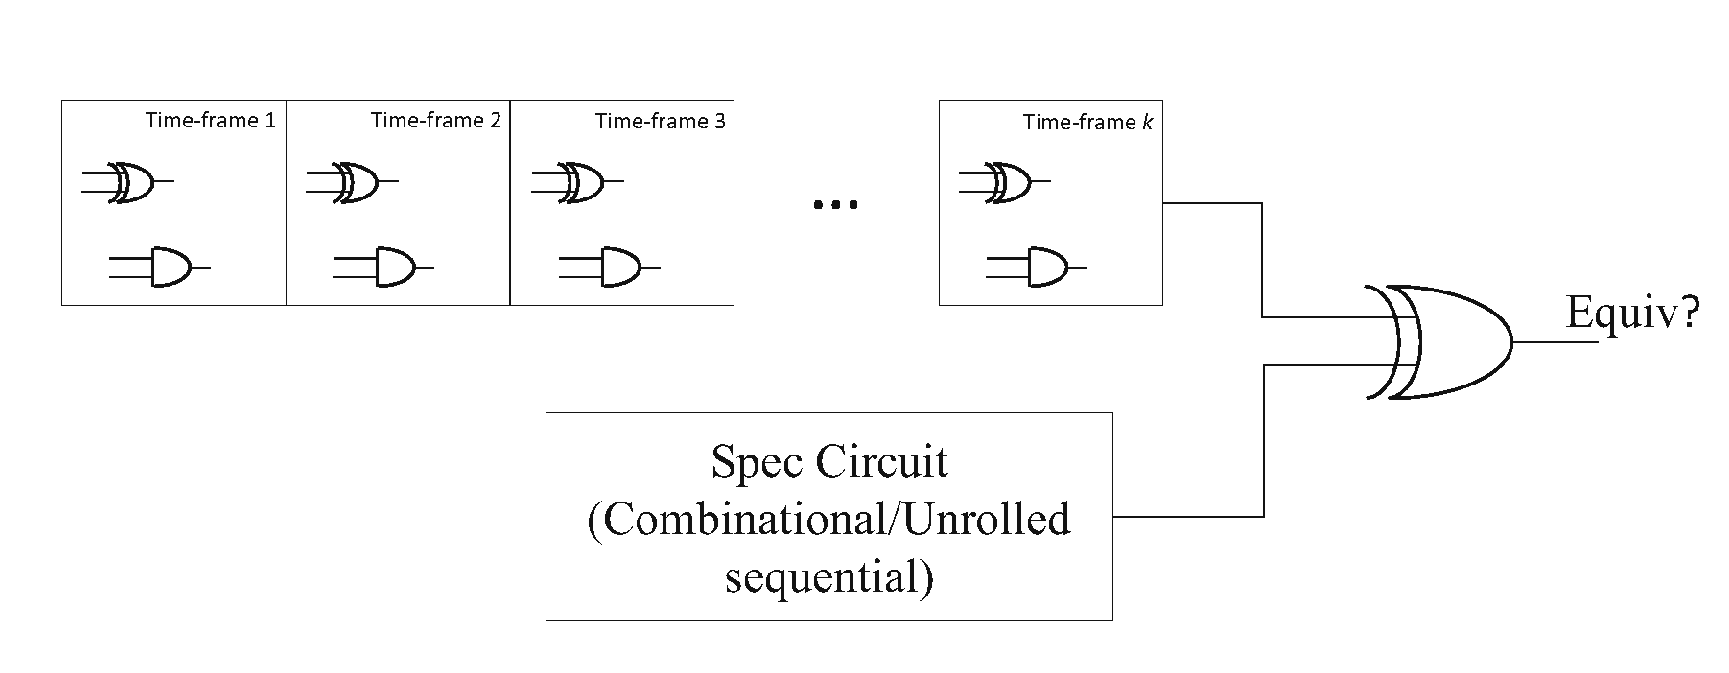
\includegraphics[width=5in]{newfig/convention.eps}
\caption{Conventional verification techniques based on bit-level unrolling and equivalence checking}
\label{fig:convention}}
\end{figure}

Conventional methods to such a sequential circuit may consist of unrolling the circuit for 
$k$ time-frames, and performing an equivalence checking between the unrolled machine and
the specification function. However, the number of gates will grow fast when doing unrolling
on bit-level. Meanwhile the structural similarity based equivalence checking techniques 
will fail when the sequential circuit is highly customized and optimized from the naive specification 
function. As a result, conventional techniques is grossly inefficient for large circuits.
Therefore, a new method based on our proposed word-level FSM traversal technique is worthy to be explored.

\section{Normal Basis Multiplier over Galois Field}
\subsection{Normal Basis}
Given a Galois field (GF) $\Fkk$ is a finite field with  $2^k$ elements and characteristic equals to 2.
Its elements can be written in polynomials of $\alpha$, when there is an irreducible polynomial $p(\alpha)$
defined.

If we use a basis $\{1,\alpha,\alpha^2,\alpha^3,\dots,\alpha^{k-1}\}$, we can easily transform polynomial representations
to binary bit-vector representations by recording the coefficients. For example,

\begin{table}[H]
\centering
\caption{Bit-vector, Exponential and Polynomial representation of
elements in  ${\mathbb{F}}_{2^4} = {\mathbb{F}}_2[x]
\pmod{x^4+x^3+1}$}
\begin{tabular}{|c|c||c|c|} 
\hline
$a_3a_2a_1a_0$ & Polynomial     &$a_3a_2a_1a_0$ & Polynomial  \\
\hline
$0000$        & $0$           & $1000$  &$\alpha^3$\\
\hline
$0001$        & $1$           & $1001$  & $\alpha^3 + 1$\\
\hline
$0010$        &  $\alpha$       & $1010$ & $\alpha^3 + \alpha$  \\
\hline
$0011$        &  $\alpha + 1$   & $1011$ &  $\alpha^3+\alpha+1$\\
\hline
$0100$        &  $\alpha^2$     &  $1100$ &  $\alpha^3 + \alpha^2$\\
\hline
$0101$        & $\alpha^2 + 1$ & $1101$  & $\alpha^3+\alpha^2+1$\\
\hline
$0110$        &  $\alpha^2 + \alpha$ & $1110$ &  $\alpha^3+\alpha^2+\alpha$\\
\hline
$0111$        & $\alpha^2+\alpha+1$ & $1111$ & $\alpha^3+\alpha^2+\alpha+1$\\
\hline
\end{tabular}
\label{table:booltogalois}  
\end{table}

Basis $\{1,\alpha,\alpha^2,\alpha^3,\dots,\alpha^{k-1}\}$ is called {\bf standard basis} (StdB), which results in
a straightforward representation for elements, and operations of elements such as addition and subtraction.
The addition/subtraction of GF elements in StdB follows the rules of polynomial addition/subtraction
where coefficients belong to $\mathbb F_2$. In other words, using the definition of {\it exclusive or} in
Boolean algebra, element $A$ add/subtract by element $B$ in StdB is defined as
\begin{align}\label{eqn:StdB}
A+B = A-B &= (a_0,a_1,\dots,a_{k-1})_{StdB} \xor (b_0,b_1,\dots,b_{k-1})_{StdB} \nonumber\\
&=(a_0\oplus b_0, a_1\oplus b_1,\dots,a_{k-1}\oplus b_{k-1})_{StdB} 
\end{align}

\subsection{Multiplication using Normal Basis}
Besides addition/subtraction, multiplication is also very common in arithmetic circuit design.
The multiplication of GF elements in $\Fkk$ in StdB follows the rule of polynomial multiplication.
However, it will result in $O(k^2)$ bitwise operations. In other words, if we implement GF multiplication
in bit-level logic circuit, it will contain $O(k^2)$ gates. When the datapath size $k$ is large,
the area and delay of circuit will be costly.

In order to lower down the complexity of arithmetic circuit design, Massey and Omura \cite{MasseyOmura} % ref 7 in RH paper
use a new basis to represent GF elements, which is called {\bf normal basis} (NB).
A normal basis over $\Fkk$ is written in the form of
\begin{equation*}
N.B. ~~~ \N = \{\beta,\beta^2,\beta^4,\beta^8,\dots,\beta^{2^{k-1}}\}
\end{equation*}
Respectively, a field element in NB representation is actually
\begin{align*}
A &= (a_0,a_1,\dots,a_{k-1})_{NB} \\
  &= a_0\beta+a_1\beta^2+\cdots+a_{k-1}\beta^{2^{k-1}} \\
  &= \sum_{i=0}^{k-1} a_i\beta^{2^i}
\end{align*}

According to the definition, a normal basis is a vector where the next entry is the square of the former one.
We note that the vector is cyclic, i.e. $\beta^{2^k} = \beta$ due to {\it Fermat's little theorem}.
{\bf Normal element} $\beta$ is an element from the field which is used to construct the normal basis,
and can be represent as a power of primitive element $\alpha$: 
\begin{equation*}
\beta = \alpha^t, ~~~ 1\leq t<2^k
\end{equation*}

The addition and subtraction of elements in NB representation are similar to equation \ref{eqn:StdB}.
However, what makes NB powerful is its property when doing multiplications and exponentiations.
The following lemmas and examples illustrate this fabulous property very well.
\begin{Lemma}[Square of NB]
\label{lem:squareNB}
In $\Fkk$, equation 
\begin{equation*}
(a+b)^2 = a^2 + b^2
\end{equation*}
has been proved. According to the \textbf{binomial theorem}, it can be extended to
\begin{align*}
&(b_0\beta + b_1\beta^2 + b_2\beta^4 + \dots + b_{k-1}\beta^{2^{k-1}})^2 \\
&= b_0^2\beta^2 + b_1^2\beta^4 + b_2^2\beta^8 + \dots + b_{k-1}^2\beta \\
&= b_{k-1}^2\beta + b_0\beta^2 + b_1\beta^4 + \dots + b_{k-2}\beta^{2^{k-1}}
\end{align*}
\end{Lemma}
This lemma concludes that the square of an element in NB equals to a simple right-cyclic shift of the bit-vector.
Obviously, StdB representation does not have this benefit.

\begin{Example}[Square of NB]
In GF $\mathbb F_{2^3}$ constructed by irreducible polynomial $x^3 + x + 1$, the standard basis is denoted as 
$\{ 1, \alpha, \alpha^2\}$ where $\alpha^3+\alpha+1=0$.
Let $\beta = \alpha^3$, then $\N = \{ \beta, \beta^2, \beta^4\}$ forms a normal basis. 
Write down element $E$ using both representations:
\begin{align*}
E &= (a_0,a_1,a_2)_{StdB} = (b_0,b_1,b_2)_{NB} \\
  &= a_0 + a_1\alpha + a_2\alpha^2 = b_0\beta + b_1\beta^2 + b_2\beta^4
\end{align*}
Compute the square of $E$ in StdB first:
\begin{align*}
E^2 &= a_0 + a_1\alpha^2 + a_2\alpha^4 \\
    &= a_0 + a_2\alpha + (a_1 + a_2)\alpha^2 \\
    &= (a_0,a_2,a_1+a_2)_{StdB}
\end{align*}
When it is computed in NB, we can make it very simple:
\begin{align*}
E^2 &= \overset{\xrightarrow{Cyclic~~shift}}{(b_0,b_1,b_2)}_{NB} \\
	&= (b_2,b_0,b_1)_{NB}
\end{align*}
\end{Example}

This example shows that convenience to use NB when computing $2^k$ power of an element.
Multiplication is a bit complicated than squaring; but when it is decomposed as bit-wise
operations, the property in lemma \ref{lem:squareNB} can be well utilized.

\begin{Example}[Bit-wise NB multiplication]
Assume there are 2 binary vectors representing 2 operands in NB over $\Fkk$: 
$A = (a_0, a_1, \dots, a_{k-1}), B = (b_0, b_1, \dots, b_{k-1})$. Note that in this example, 
by default we use normal basis representation so subscript ``NB" is skipped. Their product can also be written
as: $$C = A\times B = (c_0, c_1, \dots, c_{k-1})$$

Assume the most significant bit (MSB) of the product can be represented by a function $f_{mult}$: 
\begin{equation}
\label{eqn:multiMSB}
c_{n-1} = f_{mult}(a_0, a_1, \dots, a_{n-1}; b_0, b_1, \dots, b_{n-1})
\end{equation}
Before discussing the details of the function $f_{mult}$, we can take 
a square on both side of equation \ref{eqn:multiMSB}, i.e. $C^2 = A^2\times B^2$.
Obviously, using the property in lemma \ref{lem:squareNB}, the original second most significant bit 
becomes the new MSB because of right-cyclic shifting. 
Concretely, 
$$(c_{k-1},c_0,c_1,\dots,c_{k-2}) = (a_{k-1},a_0,a_1,\dots,a_{k-2})\times(b_{k-1},b_0,b_1,\dots,b_{k-2})$$
Note $A^2, B^2$ and $C^2$ still belong to $\Fkk$, thus as a universal function implementing MSB multiplication
over $\Fkk$, $f_{mult}$ still keeps the same. As a result, the new MSB can be written as 
\begin{equation}
\label{eqn:shiftMSB}
c_{k-2} = f_{mult}(a_{k-1}, a_0, a_1, 
\dots, a_{k-2}; b_{k-1}, b_0, b_1, \dots, b_{k-2})
\end{equation}
Similarly, if we take a square again on the new equation, we can get $c_{k-3}$.
Successively we can derive all bits of product $C$ using the same function $f_{mult}$, and the only
adjustment we need to make is to right-cyclic shift 2 operands by 1 bit each time.
\end{Example}

From above example, it is proved that a universal structure that implements $f_{mult}$ can be reused
for $k$ times in NB multiplication over $\Fkk$. Comparing to StdB, which requires distinct design 
for every bit of multiplication, NB is less costly if we can prove $f_{mult}$ will not result in 
a structure with $O(k^2)$ complexity. So our next mission is to explore the details of $f_{mult}$
to prove it will be a relatively simple design with complexity lower than $O(k^2)$.

If we want to make the complexity of $f_{mult}$ lower than $O(k^2)$, then the best choice is to try out 
linear functions. As we know, matrix multiplication can simulate all possible combinations of 
linear functions (which is also the reason it is used as basic model to simulate the behavior of a neuron
in neural network machine learning algorithms). Imagine $A$ is a $k$-bit row vector and $B$ is a $k$-bit 
column vector, then the single bit product can be written as the product of matrix multiplication
$$c_{l} = A\times C\times B$$
where $C$ is a $k\times k$ square matrix.

\begin{Definition}[$\lambda$-Matrix]
A binary $k\times k$ matrix $M$ is used to describe the bit-wise normal basis multiplication function $f_{mult}$ where
\begin{equation}
\label{eqn:def_lambda}
c_{l} = f_{mult}(A, B) = A \times M \times B^T
\end{equation}
$B^T$ denotes vector transposition. Matrix $M$ is called $\lambda$-Matrix of
$k$-bit NB multiplication over $\Fkk$.
\end{Definition} 

When taking different bits $l$ of the product in equation \ref{eqn:def_lambda}, 
we obtain a series of conjugate matrices of $M$. 
Which means instead of shifting operands $A$ and $B$, we can also shift the 
matrix.

More specifically, we denote the matrix by \emph{$l$-th $\lambda$-Matrix} as 
$$c_l = A \times M^{(l)} \cdot B^T$$
Meanwhile, the operator shifting rule in equation \ref{eqn:shiftMSB} still holds. Then we have relation 
$$c_{l-1} = A \cdot M^{(l-1)} \cdot B^T = shift(A) \cdot M^{(l)} \cdot shift(B)^T$$ which means
by right and down cyclically shifting $M^{(l-1)}$, we can get $M^{(l)}$.

\begin{Example}[NB multiplication using $\lambda$-Matrix]
Over GF $\mathbb F_{2^3}$ constructed by irreducible polynomial $\alpha^3 + \alpha + 1$, let normal element $\beta = \alpha^3$, $N = \{ \beta, \beta^2, \beta^4\}$ 
forms a normal basis. Corresponding $0$-th $\lambda$-Matrix is
\begin{equation*}
M^{(0)} = \left(
\begin{array} {lcr}
0 & 1 & 0\\
1 & 0 & 1\\
0 & 1 & 1
\end{array} \right).
\end{equation*}
i.e.,
\begin{equation*}
c_0 = (a_0\  a_1\  a_2)\left(
\begin{array} {lcr}
0 & 1 & 0\\
1 & 0 & 1\\
0 & 1 & 1
\end{array} \right)\left(
\begin{array} {lcr}
b_0\\
b_1\\
b_2
\end{array} \right)
\end{equation*}
From $0$-th $\lambda$-Matrix we can directly write down all remaining $\lambda$-Matrices:
\begin{equation*}
M^{(1)} = \left(
\begin{array} {lcr}
1 & 0 & 1\\
0 & 0 & 1\\
1 & 1 & 0
\end{array} \right)~~~~~~
M^{(2)} = \left(
\begin{array} {lcr}
0 & 1 & 1\\
1 & 1 & 0\\
1 & 0 & 0
\end{array} \right)
\end{equation*}
\end{Example}

If we generalize the definition and explore the nature of $\lambda$-Matrix, it is defined as cross-product terms from multiplication, which is 
\begin{equation}
Product~vector~C = (\sum_{i=0}^{k-1}a_i\beta^{2^i})(\sum_{j=0}^{k-1}b_j\beta^{2^j}) = \sum_{i=0}^{k-1}\sum_{j=0}^{k-1}a_ib_j\beta^{2^i}\beta^{2^j}
\end{equation}
The expressions $\beta^{2^i}\beta^{2^j}$ are referred to as cross-product terms, and can be represented by
NB, i.e.
\begin{equation}
\beta^{2^i}\beta^{2^j} = \sum_{l=0}^{k-1}\lambda_{ij}^{(l)}\beta^{2^l}, \ \ \lambda_{ij}^{(l)} \in \mathbb F_2.
\end{equation}
Substitution yields, result is an expression for l-th digit of product as showed in equation \ref{eqn:multiMSB}:
\begin{equation}
c_l = \sum_{i=0}^{k-1}\sum_{j=0}^{k-1}\lambda_{ij}^{(l)}a_ib_j
\end{equation}
$\lambda_{ij}^{(l)}$ is the entry with coordinate $(i,j)$ in $l$-th $\lambda$-Matrix.

The $\lambda$-Matrix can be implemented with XOR and AND gates in circuit design.
The very naive implementation requires $O(C_N)$ gates, where $C_N$ is the number of
nonzero entries in $\lambda$-Matrix.
There usually exists multiple NBs in $\Fkk, k>3$. If we employ a random NB, there is no mathematical
guarantee that $C_N \sim o(k)$ (symbol $o$ denotes ``strictly lower than bound"). However,
Mullin et al. \cite{mullinONB} % This citation is valid
proves that in certain GF $\mathbb F_{p^{k_{opt}}}$, there always exists at least one NB such that 
its corresponding $\lambda$-Matrix has $C_N = 2n-1$ nonzero entries. A basis with this property is
called optimal normal basis (ONB), details are introduced in appendix.

In practice, large size NB multipliers are usually designed in $\Fkk$ when ONB exists
to minimized the number of gates. So in the following part of this chapter and our experiments,
we only focus on ONB multipliers instead of general NB multipliers.


% After fixing this, add a whole-piece StdB vs NB example, list their cost as the conclusion
\subsection{Comparison between Standard Basis and Normal Basis}
At the end of this section, a detailed example is used to make a comparison between StdB multiplication
and NB multiplication.
\begin{Example}[Rijndael's finite field]
Rijndael uses a characteristic 2 finite field with 256 elements, which can also be called the GF $\mathbb F_{2^8}$.
Let us define the primitive element $\alpha$ using irreducible polynomial 
$\alpha^8+\alpha^7+\alpha^6+\alpha^4+\alpha^2+\alpha+1$. Coincidently, $\alpha$ is also a normal element,
i.e. $\beta = \alpha$ can construct a NB $\{\alpha,\alpha^2,\alpha^4,\alpha^8,\alpha^{16},\alpha^{32},\alpha^{64},
\alpha^{128}\}$.

We pick a pair of elements from the Rijndael's field: $A=(0100~1011)_{StdB} = (4B)_{StdB},~B=(1100~1010)_{StdB} = (CA)_{StdB}$.
First let us compute their product in StdB, the rule follows ordinary polynomial multiplication.

\begin{align*}
A\cdot B &= (\alpha^6+\alpha^3+\alpha+1)(\alpha^7+\alpha^6+\alpha^3+\alpha)\\
&= (\alpha^{13}+\alpha^{10}+\alpha^8+\alpha^7)+(\alpha^{12}+\alpha^9+\alpha^7+\alpha^6)+
	(\alpha^9+\alpha^6+\alpha^4+\alpha^3)\\
	&~~~+(\alpha^7+\alpha^4+\alpha^2+\alpha) \\
&= \alpha^{13}+\alpha^{12}+\alpha^{10}+\alpha^8+\alpha^7+\alpha^3+\alpha^2+\alpha
\end{align*}
Note that this polynomial is not the final form of the product because it needs to be
reduced modulo irreducible polynomial $\alpha^8+\alpha^7+\alpha^6+\alpha^4+\alpha^2+\alpha+1$.
This can be done using base-2 long division. Note the dividend and divisor are written in pseudo Boolean
vectors, not real Boolean vectors in any kind of bases.

% The folowing part is customized latex code mimicing binary long division
% Note \divrule coordinates may not reflect the intuitive column # in tabular. Adjust by urself!!!

\vspace{1cm}

\newdimen\digitwidth
\settowidth\digitwidth{0}
\def~{\hspace{\digitwidth}}


\def\divrule#1#2{%
\noalign{\moveright#1\digitwidth%
\vbox{\hrule width#2\digitwidth}}}
111010111\,\begin{tabular}[b]{@{}r@{}}
101001 \\ \hline
\big)\begin{tabular}[t]{@{}l@{}}
11010110001110 \\
111010111 \\ \divrule{0}{14}
~~111101101 \\
~~111010111 \\ \divrule{2}{12}
~~~~~111010110 \\
~~~~~111010111 \\ \divrule{5}{9}
~~~~~~~~~~~~~1
\end{tabular}
\end{tabular}
\vspace{0.5cm}

The final remainder is $1$, i.e. the product equals to 1 in StdB.

On the other hand, operands $A$ and $B$ can be written in NB as
$$A = (0010~1001)_{NB},~~B = (0100~0010)_{NB}$$
The $\lambda$-Matrix for $\mathbb F_{2}[x] \pmod{x^8+x^7+x^6+x^4+x^2+x+1}$
is
(Computation of $\lambda$-Matrix refers to appendix)
\begin{equation*}
M^{(0)} = \left(\begin{array}{lccccccr}
0 &0 &0 &0 &1 &0 &1 &1 \\
0 &0 &1 &1 &1 &1 &0 &0 \\
0 &1 &0 &0 &0 &0 &1 &0 \\
0 &1 &0 &0 &1 &1 &0 &1 \\
1 &1 &0 &1 &0 &1 &0 &0 \\
0 &1 &0 &1 &1 &0 &0 &1 \\
1 &0 &1 &0 &0 &0 &0 &0 \\
1 &0 &0 &1 &0 &1 &0 &1
\end{array}\right)
\end{equation*}
Taking matrix multiplication $c_0 = A\times M^{(0)}\times B^T$,
the result is $c_0 = 1$. Then by cyclic shifting $A$ and $B$
(or shifting $M^{(0)}$, either is applicable), we can successively
obtain other bits of product. The final answer is
$$C = (0000~0001)_{NB}$$
It is equivalent to the result in StdB.
\end{Example}

From the intuition of humans, StdB multiplication is straightforward and easier to understand
while NB is difficult to comprehend. However, if we implement both multiplications to 
hardware multipliers, it will be clear which side a circuit designer prefers.

% May consider providing details?

Mastrovito multiplier and Montgomery multiplier are 2 common designs
of GF multipliers using StdB. As a naive implementation of GF multiplication,
Mastrovito multiplier uses most number of gates:
$k^2$ AND gates plus $k^2-\Delta$ XOR gates \cite{Mastrovito}. Montgomery multiplier 
applies lazy reduction techniques and results in a better latency performance, while the number of gates are about
the same with Mastrovito multiplier:
$k^2$ AND gates plus $k^2-k/2$ XOR gates \cite{Montgomery}. 
Concretely, typical design of Mastrovito multiplier consists of 218 logic gates, while 
Montgomery multiplier needs 198 gates. However, the NB multiplier reuses the $\lambda$-Matrix 
logic, so this component will only need to be implemented for once. 
Consider the definition of matrix multiplication, it needs $C_N$ AND gates to apply 
bit-wise multiplication and $C_N-1$ XOR gates to sum them up. The number of nonzero entries
in the $\lambda$-Matrix can be counted: $C_N = 27$.
As a result, the most naive NB multiplier design (or Massey-Omura multiplier \cite{MasseyOmura})
contains 53 gates in total, which is a great saving in area cost comparing to StdB multipliers.